\section{Login and slides}
\begin{frame}[fragile]
  \frametitle{Login and slides}

  \begin{itemize}
  \item If you do not have an account on Hadoop cluster, use yubikey:
    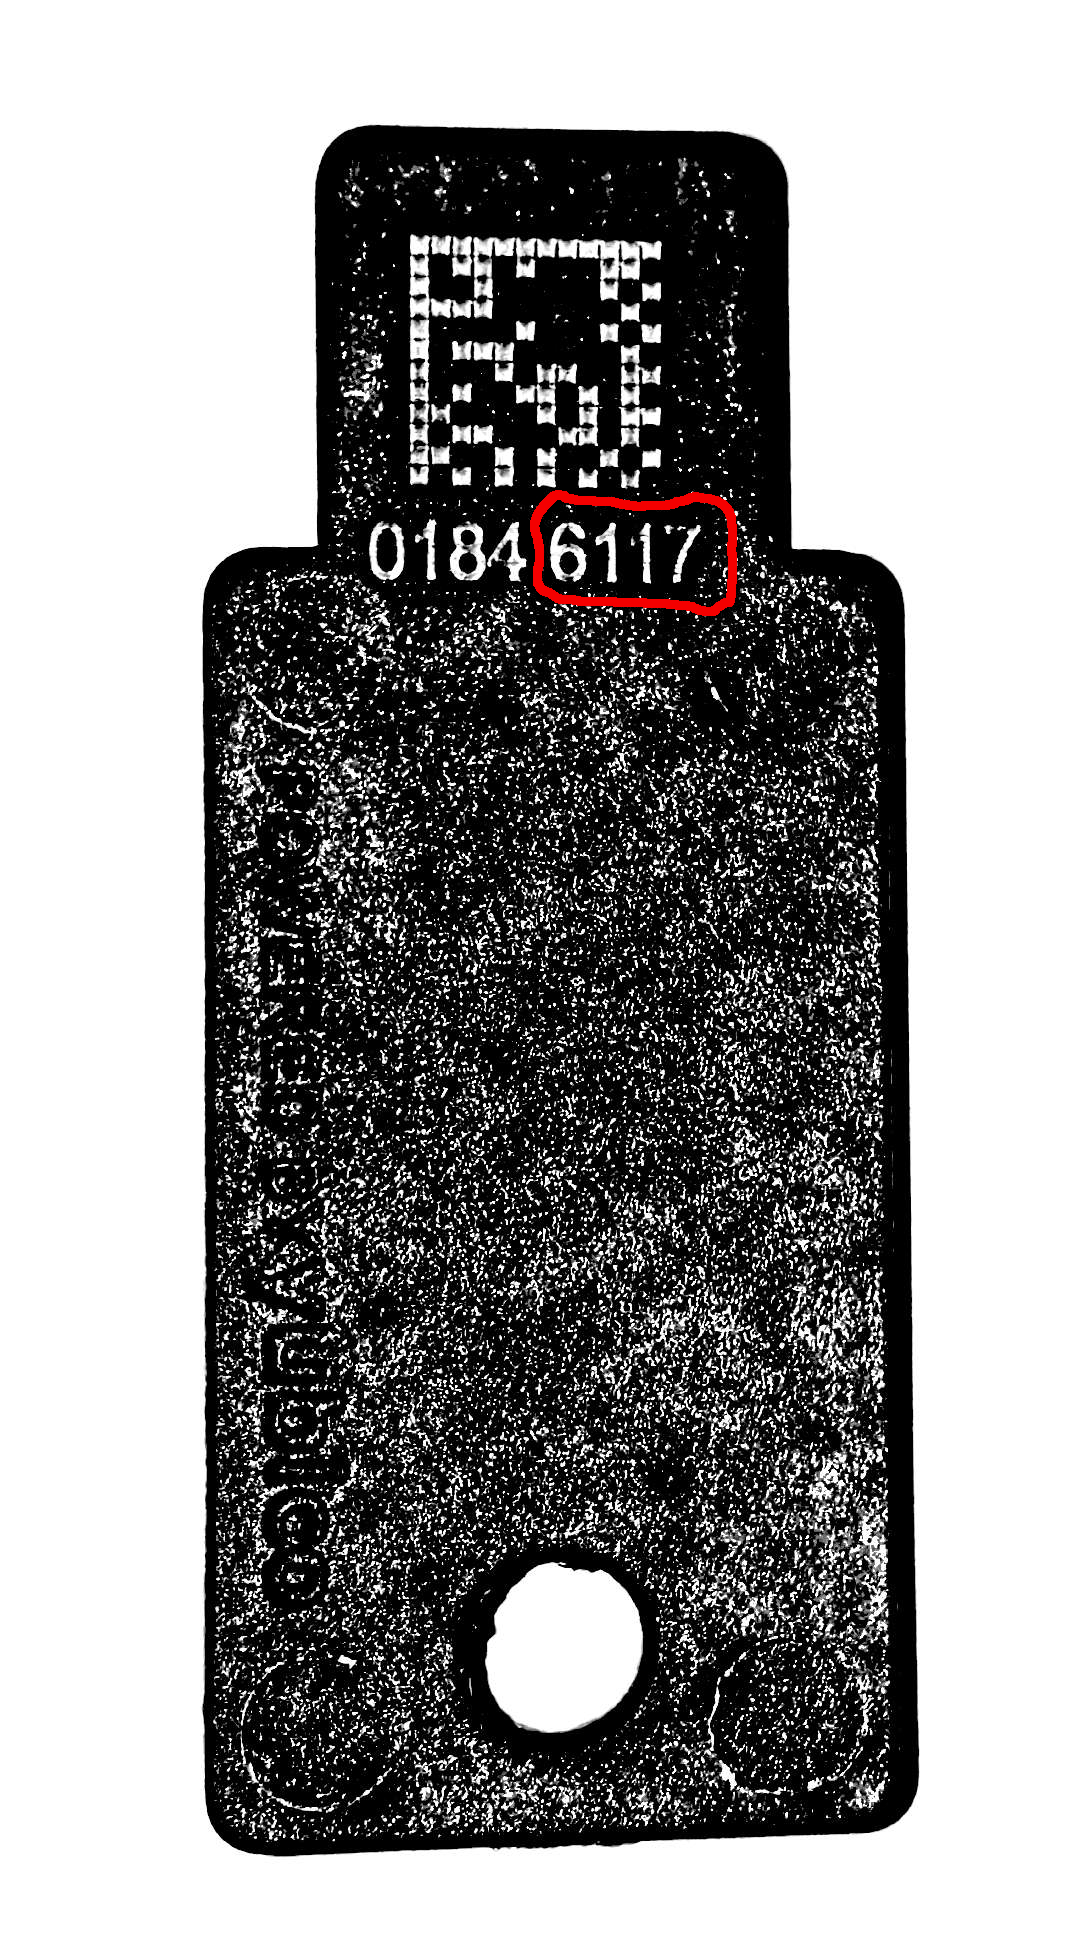
\includegraphics[width=1.5cm]{icons/yubikey1a.jpg}
    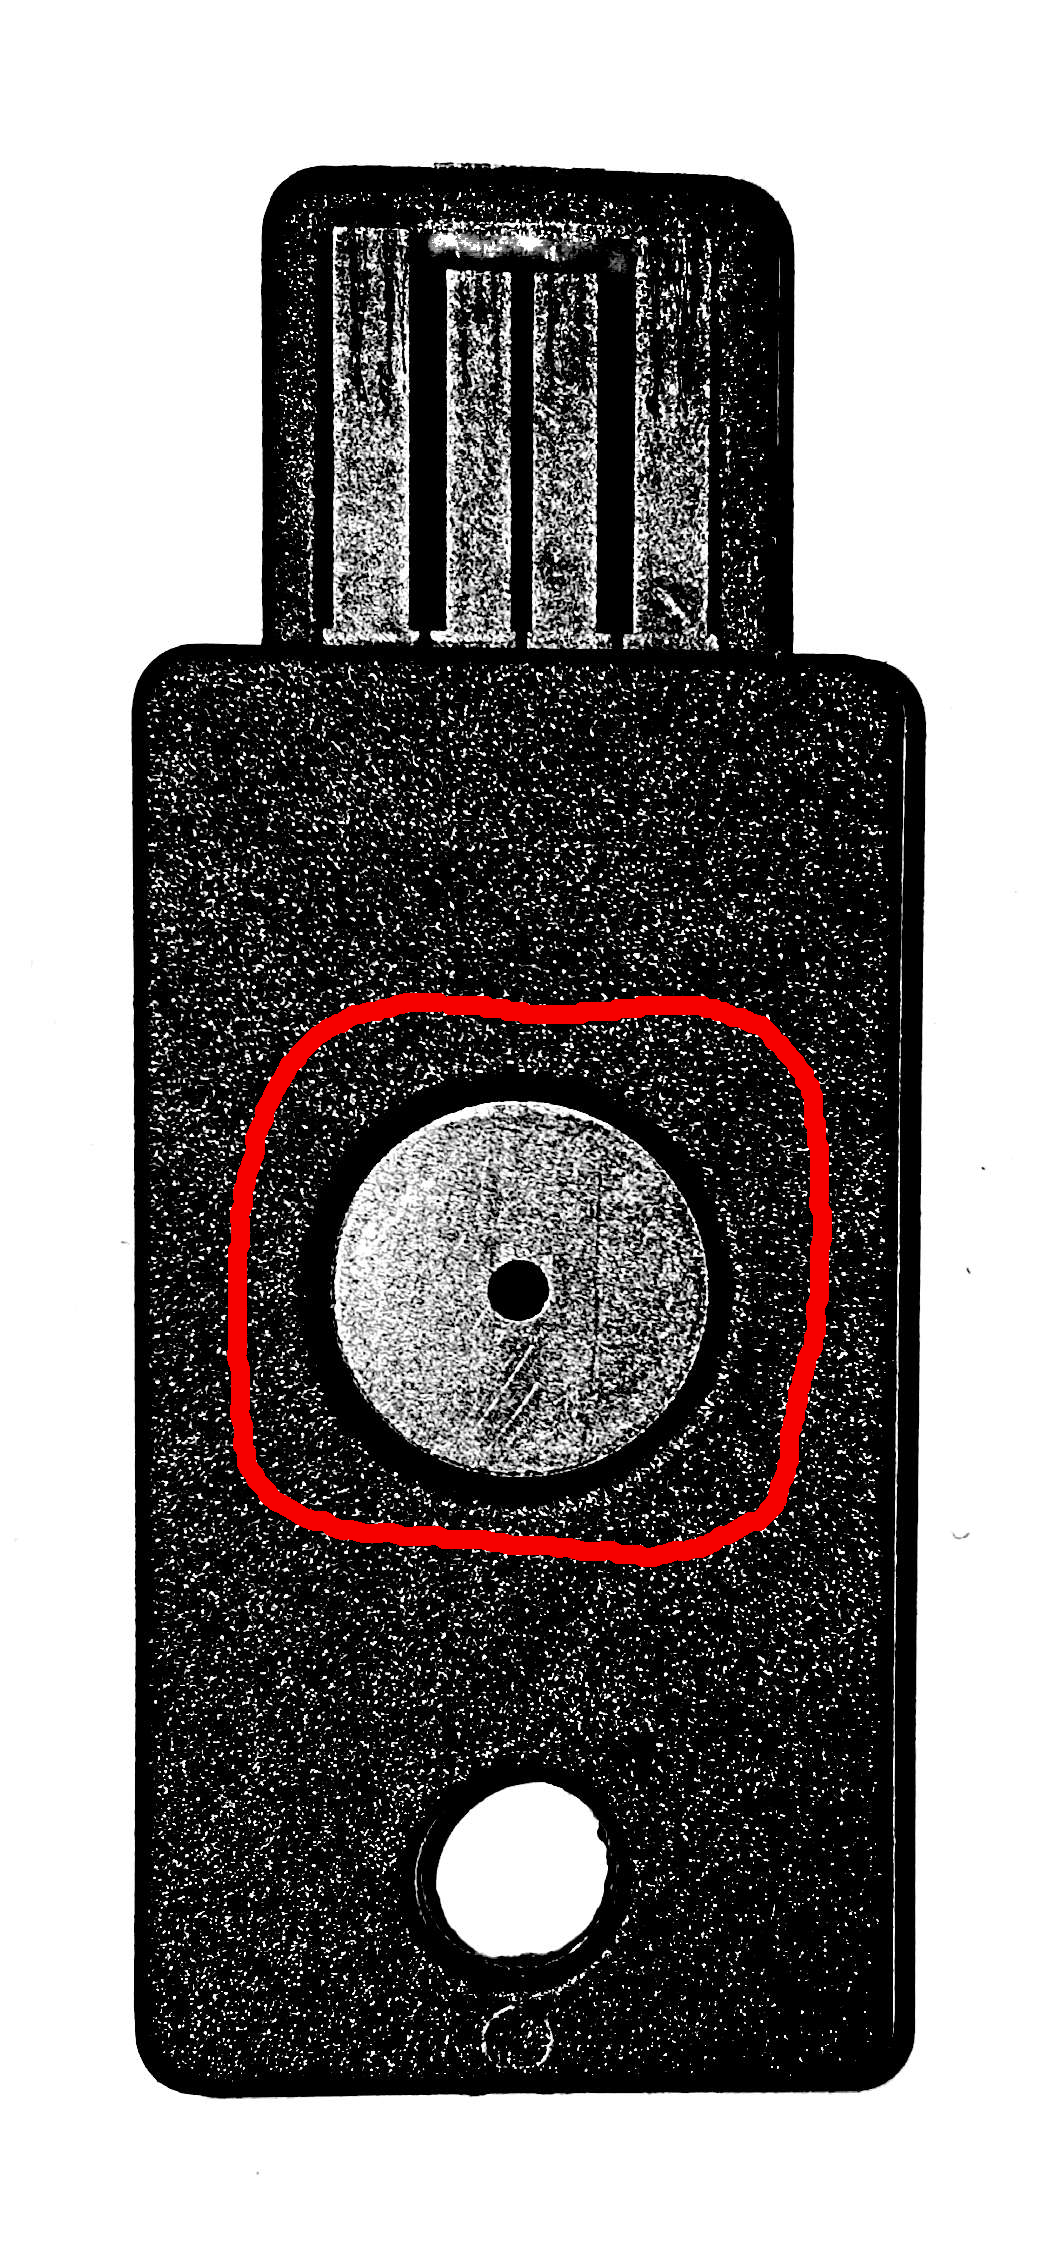
\includegraphics[width=1.3cm]{icons/yubikey2a.jpg}
    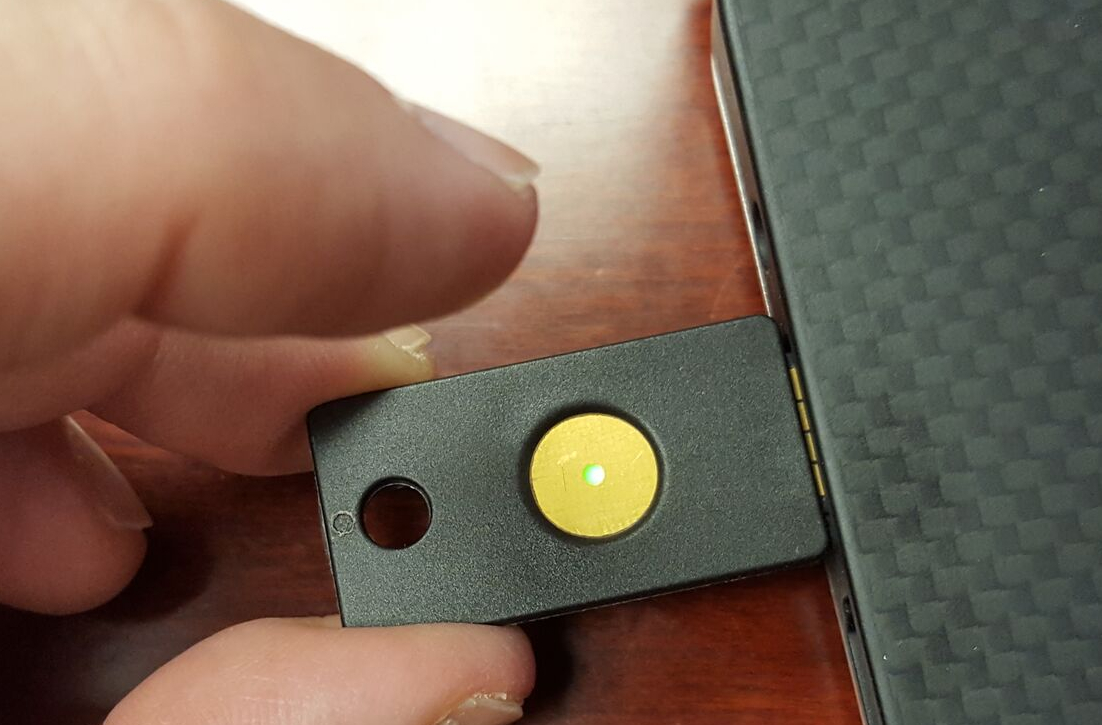
\includegraphics[width=3.3cm]{icons/yubikey3a.jpg}
  \item Use last 4 digits of yubikey as part of userid:
    {\color{mycolorcli}
\begin{verbatim}
ssh -Y rccguest<XXXX>@hadoop.rcc.uchicago.edu
\end{verbatim}
    }
  \item Push the button when asked for password
  \item If you have an account on Hadoop cluster
    {\color{mycolorcli}
\begin{verbatim}
ssh -Y <username>@hadoop.rcc.uchicago.edu
\end{verbatim}
    }
  \item To get slides and labs, point the browser to:
    {\tiny
      {\color{mycolorcli}
\begin{verbatim}
https://git.rcc.uchicago.edu/ivy2/Graham_Introduction_to_Hadoop
\end{verbatim}
      }
    }
  \item After logging into Hadoop cluster, get code and slides:
    {\tiny
      {\color{mycolorcli}
\begin{verbatim}
git clone https://git.rcc.uchicago.edu/ivy2/Graham_Introduction_to_Hadoop.git
\end{verbatim}
      }
    }
  \end{itemize}
\end{frame}

\subsection{2fa}
\begin{frame}[fragile]
  \frametitle{Login and slides: 2fa}
  \begin{itemize}
  \item Since the end of last year, there is an extra extremely annoying security complication: 
    {\color{mycolordef}2-factor authentication}.
  \item You need to follow the instructions on {\color{mycolorcli}\verb|https://cnet.uchicago.edu/2FA/index.htm|} 
    to enroll in 2-factor authentication.
    Another useful related page: {\color{mycolorcli}\verb|https://2fa.rcc.uchicago.edu|}.
  \item You would need to install an application on your phone so that when you try to connect to midway, 
    you get notification on your phone to which you need to respond
  \item If you do not have a phone or travelling abroad, 
    you can get a set of passcodes that you can type instead, each time using the next passcode from the list and periodically
    getting a new list once you use all the numbers from there.
  \end{itemize}
\end{frame}


